% AI-Intent: Conceptual Modeling for Accountable Multi-Agent AI Systems
% Springer LNCS format for ER 2026 (Conceptual Modeling Conference)

\documentclass[runningheads]{llncs}

\usepackage[T1]{fontenc}
\usepackage{graphicx}
\usepackage{booktabs}
\usepackage{amsmath}
\usepackage{amssymb}
\usepackage{listings}
\usepackage{xcolor}
\usepackage{hyperref}
\usepackage{tikz}
\usetikzlibrary{arrows.meta, positioning, shapes.geometric, fit}
\usepackage{comment}
\usepackage{tabularx}
\usepackage{tablefootnote}

\lstset{
  basicstyle=\ttfamily\small,
  keywordstyle=\color{blue}\bfseries,
  stringstyle=\color{red!70!black},
  commentstyle=\color{green!50!black}\itshape,
  breaklines=true,
  frame=single,
  numbers=left,
  numberstyle=\tiny\color{gray},
  backgroundcolor=\color{gray!5},
  captionpos=b,
  aboveskip=8pt,
  belowskip=8pt,
}

\begin{document}

\title{AI-Intent: A Conceptual Modeling Framework\\
for Accountable Multi-Agent AI Systems}

\titlerunning{AI-Intent: A Conceptual Modeling Framework}

\begin{comment}
\author{Wolfgang Maa\ss\inst{1} \and Iris Reinhartz-Berger\inst{2}}
\authorrunning{W.~Maa\ss{} and I.~Reinhartz-Berger}
\institute{German Research Center for Artificial Intelligence (DFKI)\\
and Saarland University, Saarbr\"ucken, Germany\\
\email{wolfgang.maass@dfki.de}
\and University of Haifa, Haifa, Israel\\
\email{iris@is.haifa.ac.il}}
\end{comment}

\author{Anonymous Author(s)}
\authorrunning{Anonymous Author(s)}
\institute{Anonymous Institution(s)\\
\email{anonymous@domain.com}}

\maketitle

\begin{abstract}
Existing agent-oriented conceptual modeling frameworks were designed
for software components with deterministic execution semantics. Applied
to language model agents, whose outputs are governed by
probabilistic text generation and natural-language inputs,
these frameworks lack three governance constructs that accountability
requires: a means to \emph{declare} the legitimate action space of each
agent as a binary boundary; a means to \emph{enforce} negative
obligations at runtime via an external component rather than relying on
agent self-compliance; and a means to treat inter-agent communication as
\emph{auditable evidence}.

To address these gaps, we introduce \textsc{AI-Intent},
a conceptual modeling framework organized into three governance pillars.
The \textbf{\textit{Declaration}} pillar makes the legitimate action
space of each agent explicit before execution through \textit{Mandates}
that encode decision rights, boundary constraints, permitted capabilities,
and risk policies. The \textbf{\textit{Enforcement}} pillar operationalizes
those Mandates at runtime through a Compliance Agent that intercepts
every \textit{Proposed Action} and evaluates it against applicable
constraints before delivery, enforcing norms externally rather than relying on agent self-compliance. The
\textbf{\textit{Auditability}} pillar derives a structured, durable
record from every session, capturing what was approved as well as what was blocked and on what grounds.

The framework is evaluated through a reference implementation for
private investment advisory, a domain that combines multiple specialized
agents and clear regulatory requirements (MiFID~II). Across 190
evaluation sessions, boundary violation containment averaged 97.9\%
with zero forced-pass occurrences. Audit trace completeness depends,
however, on the instruction-following capability of the deployed model.

\keywords{Multi-Agent Systems \and Conceptual Modeling \and
Language Model Agents \and Accountability \and Governance}
\end{abstract}

%=====================================================================
\section{Introduction}
\label{sec:introduction}
%=====================================================================

Language model-based agents are rapidly moving from research prototypes
to production systems that support consequential decisions in finance,
healthcare, and enterprise operations~\cite{wang2024survey,xi2023rise}.
Unlike traditional software components, whose runtime behavior is fully
determined by source code, language model agents generate outputs through
probabilistic text generation that is governed by natural language inputs,
training data, and model parameters. When multiple such agents collaborate,
delegating sub-tasks, synthesizing partial results, and producing joint
recommendations, questions arise that existing
conceptual models are not equipped to answer: what was each agent
supposed to do, whether it stayed within its designated scope, and why
a particular output was produced.

Addressing these questions requires revisiting the foundations. Conceptual modeling frameworks for multi-agent systems have a rich
history~\cite{yu2011social,bresciani2004tropos,wooldridge2000gaia}, modeling agents in terms of goals, capabilities, roles, and inter-agent
dependencies to provide formal foundations for requirements analysis and
system design. However, these frameworks share an assumption that their
target components have deterministic or rule-governed execution semantics.
This assumption does not hold for language model agents, giving rise to
three modeling gaps.

\medskip
\noindent\textbf{Gap~1: Intent boundary versus goal satisfaction.}
Traditional goal models, such as $i^*$ and Tropos, treat goal
satisfaction as graded~\cite{yu2011social}: softgoals can be partially
achieved, contributing positively or negatively to parent goals. For
language model agents, the relevant construct is not graded goal
satisfaction but a binary \emph{sortal boundary}: a request either falls
within the agent's legitimate scope or it does not. An equity analyst
agent recommending gold at 35\% allocation has not partially satisfied
its goal; it has transgressed its mandate scope.

\medskip
\noindent\textbf{Gap~2: Negative obligations as runtime-enforceable
constraints.} Normative frameworks and deontic logic provide
well-developed accounts of obligation, permission, and
prohibition~\cite{vonwright1951essay,governatori2005meeting,boella2006introduction}. In classical normative agent architectures,
norms are represented declaratively and reasoned about by the agent
itself~\cite{dignum1999autonomous}. For language model agents, however,
agents may acknowledge a constraint and then violate it, or construct
superficially plausible justifications for
exceptions~\cite{huang2023selfcorrect}. The modeling challenge is
therefore to represent negative obligations in a form that an
\emph{external} enforcement component can evaluate, rather than one
that relies on agent self-compliance.

\medskip
\noindent\textbf{Gap~3: Communication as audit evidence.} Existing agent
communication models, such as FIPA-ACL~\cite{fipa2002}, specify message
syntax and semantics but treat communication logs as an optional
engineering concern. Regulatory frameworks for AI systems, including
the EU AI Act~\cite{euaiact2024} and MiFID~II~\cite{mifid2014}, require
that every consequential decision be traceable to its inputs. Meeting
this requirement demands that communication logging be a \emph{structural
property} of the conceptual model, not an add-on.

\medskip
To address these gaps, we propose \textsc{AI-Intent}, organized into
three pillars, one per gap. \textbf{\textit{Declaration}} introduces the
\textit{Mandate}, a first-class artifact encoding an agent's binary action
boundary, decision rights, capabilities, and risk policies.
\textbf{\textit{Enforcement}} introduces \textit{Intent Enforcement}, a
mandatory gatekeeper that evaluates every \textit{Proposed Action} against
the applicable Mandate and \textit{Regulatory Framework}, producing a
\textit{Compliance Verdict} before delivery. \textbf{\textit{Auditability}}
derives an \textit{Accountability Trace} from the \textit{Log Entry} of
every verdict, recording what was approved as well as what was blocked and
on what grounds.

\noindent\textbf{Nature and scope of the contribution.} We state at the
outset what AI-Intent is and is not. It is \emph{not} a new modeling
language, nor an extension to the syntax of an existing one; it is a
domain-independent \emph{conceptual model} -- governance constructs with
their metamodel relationships and well-formedness conditions, grounded in
the Unified Foundational Ontology (UFO)~\cite{guizzardi2005ontological}
and rendered in OntoUML. It \emph{augments} rather than replaces existing
agent-oriented languages: where $i^*$, Tropos, GAIA, and NMAS model what
agents want, can, and should do, AI-Intent adds the orthogonal constructs
needed to declare, enforce, and audit what an agent \emph{must not} do.
The paper is accordingly structured as a gap analysis
(Section~\ref{sec:background}) followed by the constructs that close those
gaps (Section~\ref{sec:framework}).

To evaluate AI-Intent, we have developed a reference implementation for private
investment advisory, a domain combining multiple
specialized agents and regulatory requirements.
Evaluated across 190 sessions, spanning 10
independent runs, 19 test cases, and four adversarial disposition
presets, boundary violation containment averaged 97.9\% with zero
forced-pass occurrences, including under adversarial agent dispositions.
Even under a neutral disposition preset in which agents received
no adversarial modification, the materials agent violated its allocation
cap on the first attempt in 12.9\% of sessions, motivating external
enforcement as a structural modeling requirement.
%rather than an engineering convenience.

The remainder of the paper is organized as follows. Section~\ref{sec:background}
reviews existing agent-oriented modeling frameworks. Section~\ref{sec:framework}
presents the AI-Intent framework across its three pillars. Section~\ref{sec:evaluation}
reports the empirical evaluation, while Section~\ref{sec:discussion}
discusses the results. Section~\ref{sec:conclusion} concludes and
identifies directions for future work.

%=====================================================================
\section{Background and Related Work}
\label{sec:background}
%=====================================================================

We apply an explicit selection criterion to a broad landscape. We treat
as directly related any work that proposes \emph{modeling constructs} for
agent governance (Section~\ref{sec:aomodeling}); multi-agent
implementation frameworks (Section~\ref{sec:mala}) and AI-governance
policy work (Section~\ref{sec:aigov}) are surveyed as deployment substrate
and normative context, not as competing modeling contributions.

\subsection{Agent-Oriented Conceptual Modeling}
\label{sec:aomodeling}

To identify what existing frameworks lack, the present section examines
four influential modeling approaches through the lens of the three
governance gaps introduced above: $i^*$~\cite{yu2011social},
Tropos~\cite{bresciani2004tropos}, GAIA~\cite{wooldridge2000gaia}, and
Normative Multi-Agent Systems (NMAS)~\cite{boella2006introduction}. We
note the terminological distinction the taxonomy warrants: $i^*$ and
Tropos are \emph{goal}-oriented, whereas GAIA and NMAS are
\emph{agent}-oriented in the stricter sense; we group them here because
each supplies constructs a governance model must either reuse or replace.

\textbf{The $i^*$ framework}~\cite{yu2011social} models actors with
goals, tasks, resources, and softgoals connected by contribution links.
Its softgoal construct explicitly supports partial satisfaction: a design
decision may contribute positively or negatively to a softgoal. This
graded semantics is well suited to modeling design trade-offs but is
inappropriate for mandate boundaries, where violations are categorical
rather than a matter of degree.
\textbf{Tropos}~\cite{bresciani2004tropos} extends $i^*$ into a full
software development methodology, introducing plans as sequences of
activities satisfying goals and capability models linking agents to the
plans they can execute. The framework provides no construct for
prohibitions: it specifies what agents can and should do, not what they
must not do.

\textbf{GAIA}~\cite{wooldridge2000gaia} provides role models with
permissions, responsibilities, activities, and protocols. Its permission
construct is the closest existing analog to boundary constraints: a
role's permissions define the actions it is authorized to take. However,
permissions are granted at modeling time and assumed to hold at runtime;
no mechanism exists for verifying that an agent stays within its
permissions during execution. For agents with deterministic behavior,
this assumption is safe; for language model agents, it is not.

\textbf{Normative Multi-Agent Systems~(NMAS)}~\cite{governatori2005meeting,boella2006introduction,dignum1999autonomous} address obligation and
prohibition more directly, employing deontic operators for obligation
($\mathbf{O}$), permission ($\mathbf{P}$), and
prohibition~($\mathbf{F}$)~\cite{vonwright1951essay}. Defeasible deontic
logic~\cite{governatori2005meeting} allows norms to have exceptions and
to be defeated by stronger norms, which is appropriate for complex
multi-stakeholder settings. However, these approaches assume agents that
deliberate over norms, evaluating their intended actions against
applicable norms before acting. Language model agents do not deliberate
in this sense; they generate text that may or may not comply with norms,
depending on how those norms are represented in the input specification
and how reliably the model follows
instructions~\cite{huang2023selfcorrect}.

Table~\ref{tab:comparison} captures this analysis systematically and
contrasts it with the recent trustworthy-agent frameworks
(Section~\ref{sec:aigov}) and with AI-Intent. Across the four modeling
frameworks, coverage is partial and uneven: $i^*$ and Tropos represent
neither prohibitions nor scope boundaries; GAIA adds permissions but
cannot verify them at runtime; NMAS closes the representational gap on
prohibitions but relies on agent self-deliberation for enforcement, an
assumption that fails for non-deterministic generators. The recent
trustworthy-agent frameworks supply runtime auditing and provenance but
no declarative modeling constructs for scope, prohibition, or risk. Only
AI-Intent covers all eight capabilities, which is the gap the framework
is designed to close.

\vspace{-14pt}

\begin{table}
\centering
\caption{Comparative analysis of agent governance modeling capabilities,
contrasting the four agent-oriented modeling frameworks and the recent
runtime trustworthy-agent frameworks (Trust.\ MAS: Alqithami's
AAF~\cite{alqithami2025adaptive}, verifiability-first
agents~\cite{gupta2025verifiability}) with AI-Intent. \checkmark~= fully
expressible; $\circ$~= partial/with significant extensions; $\times$~=
not expressible without framework revision. Trust.\ MAS are runtime
mechanisms, not modeling languages; marks reflect what each represents as
an explicit construct. \emph{Model operativity} denotes runtime injection
of mandate constraints into the deployed model's input specification.}
\label{tab:comparison}
\setlength{\tabcolsep}{4pt}
\resizebox{\textwidth}{!}{%
\begin{tabular}{@{}lcccccc@{}}
\toprule
\textbf{Capability} & \textbf{$i^*$} & \textbf{Tropos} &
\textbf{GAIA} & \textbf{NMAS} & \textbf{Trust.\ MAS} &
\textbf{AI-Intent} \\
\midrule
Intent scope (binary sortal boundary) & $\times$ & $\times$ &
    $\circ$ & $\circ$ & $\times$ & \checkmark \\
Negative obligations (prohibitions)   & $\times$ & $\times$ &
    $\circ$ & \checkmark & $\times$ & \checkmark \\
Quantitative risk parameters          & $\times$ & $\times$ &
    $\times$ & $\circ$ & $\times$ & \checkmark \\
Runtime constraint enforcement        & $\times$ & $\times$ &
    $\times$ & $\circ$ & $\circ$ & \checkmark \\
External Compliance Agent             & $\times$ & $\times$ &
    $\times$ & $\times$ & $\circ$ & \checkmark \\
Audit-native communication            & $\times$ & $\times$ &
    $\times$ & $\times$ & \checkmark & \checkmark \\
Compliance history in trace           & $\times$ & $\times$ &
    $\times$ & $\times$ & $\circ$ & \checkmark \\
Model operativity (runtime injection) & $\times$ & $\times$ &
    $\times$ & $\times$ & $\times$ & \checkmark \\
\bottomrule
\end{tabular}%
}
\end{table}

\vspace{-20pt}

\subsection{Multi-Agent Language Model Architectures}
\label{sec:mala}

Where agent-oriented modeling frameworks lack runtime enforcement,
current multi-agent language model architectures lack formal modeling
altogether. AutoGen~\cite{wu2023autogen}, CrewAI~\cite{crewai2024}, and
LangGraph~\cite{langgraph2024} enable language model agents to
collaborate through role specification, tool invocation, and
interaction-based task coordination, but represent agent roles primarily
as natural-language descriptions with no formal constraint semantics or
runtime verification. The Model Context Protocol
(MCP)~\cite{anthropic2024mcp} standardizes communication between
language model applications and external tools through a client-server
architecture, providing interoperability but not governance. AI-Intent
builds on MCP's communication substrate and adds the governance layer
that MCP lacks.

Output filtering systems, such as NeMo
Guardrails~\cite{rebedea2023nemo} and Constitutional
AI~\cite{bai2022constitutional}, address output compliance for
individual models through input and output filtering and self-assessment
mechanisms. These systems enforce constraints on single-agent outputs
but do not model inter-agent accountability: they cannot trace a
multi-agent decision to its constituent sub-agent outputs, do not
maintain compliance histories across revision cycles, and do not produce
structured audit artifacts. AI-Intent shares the underlying motivation,
namely constraint enforcement on non-deterministic outputs, but operates
at the multi-agent communication level rather than at the single-model
output level.

\subsection{AI Governance and Accountability}
\label{sec:aigov}

Existing accountability frameworks address individual model
decisions~\cite{arrieta2020explainable} and dataset
documentation~\cite{gebru2021datasheets,mitchell2019model}, but fall
short of \emph{multi-agent accountability}: tracing a joint decision
back to the sub-agent outputs and constraint evaluations that produced
it. The EU AI Act~\cite{euaiact2024} classifies AI systems by risk
tier and mandates transparency, auditability, and human oversight for
high-risk applications. Financial AI systems are subject to additional
requirements under MiFID~II, requiring that investment recommendations
be traceable to their inputs and that conflicts of interest be disclosed.
Neither regulatory instrument specifies how traceability is to be
achieved in systems where a decision is the product of multiple
collaborating agents.

A recent line of work targets trustworthiness and accountability in
language model agent systems directly, and is the closest state of the
art. Alqithami's Adaptive Accountability Framework~\cite{alqithami2025adaptive}
is a runtime layer that records verifiable interaction provenance,
detects distributional change points in streaming traces, and attributes
responsibility via a causal influence graph, targeting \emph{emergent}
norm violations at scale. Verifiability-first
designs~\cite{gupta2025verifiability} embed lightweight audit agents and
attestations to minimize time-to-detect misalignment, while governance
frameworks for multi-agent AI~\cite{pujari2024ethical,techrxiv2026unified,ieee2025trustworthy}
treat accountability failures as governance-design problems and propose
evaluation and policy scaffolding. These works share AI-Intent's
motivation but differ in level: they are runtime, policy, or evaluation
\emph{mechanisms}, whereas AI-Intent is a \emph{conceptual model} that
specifies the constructs such mechanisms leave implicit -- a declared
per-agent action boundary, an external enforcement role, and an audit
artifact derived as a well-formedness condition. Where they detect or
attribute violations \emph{a posteriori} from observed traces,
AI-Intent's enforcement intercepts each Proposed Action \emph{before}
delivery. The directions are complementary: a system could realize
AI-Intent's constructs and adopt~\cite{alqithami2025adaptive}'s
attribution for residual emergent behaviors that per-message enforcement
does not cover.

Enterprise architecture standards and Service-Oriented Architecture
compliance logging provide audit trails as infrastructure services.
By design, such logs record what happened; they are not first-class
elements that constrain system behavior at runtime. AI-Intent
addresses this distinction: in \textit{AI-Intent}, the \textit{Accountability Trace} is a
structural model component whose existence is a well-formedness
condition, and the \textit{Compliance Verdict} attached to each message is a
metamodel relationship rather than a log entry.

%=====================================================================
\section{The AI-Intent Framework}
\label{sec:framework}
%=====================================================================

AI-Intent is a metamodel of governance constructs, their relationships,
and well-formedness conditions, independent of any implementation. This
section states its ontological commitments (Section~\ref{sec:ontology})
and then its constructs, grouped into three pillars
(Section~\ref{sec:pillars}), distinguishing throughout constructs
\emph{derived from} UFO (which inherit its formal properties) from
\emph{design choices} layered on top; Table~\ref{tab:ufo} summarizes this
mapping and the precise extent of the framework's dependence on UFO.

\subsection{Core Principles and Ontological Commitments}
\label{sec:ontology}

AI-Intent adopts the following ontological commitments, grounded in the
Unified Foundational Ontology (UFO)~\cite{guizzardi2005ontological} and
standard deontic
semantics~\cite{vonwright1951essay,governatori2005meeting}.

\textbf{Agents as intentional objects.} Following UFO, agents are
treated as intentional objects with dispositions to act in certain ways.
An agent's Mandate specifies the intended disposition: the range of
behaviors the agent is authorized to exhibit, the boundaries it must not
cross, and the risk parameters within which it must operate.

\textbf{Intent scope as a sortal boundary.} We use \emph{sortal} in its
established ontological sense~\cite{gupta1980common}: a sortal universal
supplies a principle of identity and individuation, determining for any
candidate whether it \emph{is or is not} an instance of the
type~\cite{guizzardi2005ontological}, and is therefore inherently binary
rather than graded. The intent scope
in the Mandate is not a goal, which admits degrees of satisfaction, but a
natural-language specification delineating such a sortal boundary: the
category of situations to which the agent's competence applies, which
partitions the query space into in-scope and out-of-scope regions. We
adopt the sortal reading rather than a mere subtype predicate because its
identity criterion makes ``the same kind of request'' well defined across
the paraphrastic variation typical of language model queries.

\textbf{Boundary constraints as prohibitions.} Following deontic
logic~\cite{vonwright1951essay}, the boundary constraints encoded in the
Mandate are prohibitions of the form $\mathbf{F}(\phi)$: the agent is
forbidden from producing outputs satisfying predicate $\phi$. Risk
parameters provide quantitative instantiations, for example
$\mathbf{F}(\mathit{allocation} > 0.15)$ for a 15\% cap. Unlike NMAS
norms, these prohibitions are evaluated by the Intent Enforcement
component against every Proposed Action before delivery, rather than
reasoned about by the agent itself.

\textbf{Intent Enforcement as a structural role.} Intent Enforcement is
not an optional component but a central element of the framework. It
makes prohibitions operative at runtime. A framework that can represent
prohibitions in a Mandate but provides no enforcement mechanism cannot
guarantee that those prohibitions hold on any given agent output.

\textbf{Communication as evidence.} Every inter-agent action is a
time-stamped, non-repeatable UFO \emph{event} that produces a Compliance
Verdict, recorded as a Log Entry and aggregated into the Accountability
Trace.

\medskip
\noindent\textbf{Dependence on UFO.} AI-Intent \emph{depends on} UFO for
the ontological \emph{categorization} of its constructs and the resulting
entailments, but does \emph{not} require a UFO reasoner at runtime: the
reference implementation operationalizes the categories without
ontological inference. Three constructs are genuinely UFO-derived.
Treating each inter-agent action as an \emph{event} entails that it is
time-indexed and non-repeatable, licensing its use as non-repudiable
evidence; treating the Accountability Trace as a \emph{situation} (a UFO
truthmaker aggregating events) makes it a derived first-class object
rather than a side-effect log; treating agents as \emph{intentional
objects with dispositions} lets a Mandate constrain a disposition-to-act
rather than an observed behavior. By contrast, the Mandate's internal
structure, the external Compliance Agent, and the quantitative risk
parameters are design choices layered on top. The value of the UFO
grounding is clearest in the counterfactual: a non-UFO design would
plausibly have produced (i)~the Mandate as a goal-set rather than a
normative description, reintroducing the graded satisfaction that Gap~1
rejects; (ii)~the audit trail as an infrastructure artifact rather than a
derived situation, forfeiting the well-formedness guarantee of
Section~\ref{sec:pillars}; and (iii)~messages permitted to exist without
an attached verdict, breaking communication-as-evidence. The three
UFO-derived commitments are precisely what exclude these alternatives.
Table~\ref{tab:ufo} records the full mapping, including the OntoUML
stereotype and the reference-implementation realization of each construct.

\vspace{-6pt}
\newcommand{\uml}[1]{\guillemotleft #1\guillemotright}
\begin{table}
\centering
\caption{Grounding of AI-Intent constructs in UFO. \emph{Src}
distinguishes UFO-\emph{der}ived commitments (which inherit formal
entailments) from \emph{des}ign choices layered on top; the
\emph{Realization} column gives the corresponding element of the
reference implementation.}
\label{tab:ufo}
\begin{tabularx}{\textwidth}{@{}p{2.5cm} p{4.1cm} c X@{}}
\toprule
\textbf{Construct} & \textbf{UFO category / OntoUML stereotype} &
\textbf{Src} & \textbf{Realization in reference impl.} \\
\midrule
Principal & Intentional object, \uml{kind} & des &
    Human/institutional owner (config) \\
Agent & Intentional object w/ dispositions, \uml{kind} & der &
    Orchestrator $+$ three sub-agents \\
Mandate & Normative description (\emph{not} a goal) & des &
    Pydantic schema injected into input spec \\
Intent scope & Sortal universal & der &
    Natural-language scope string \\
Boundary constraint & Negative duty, \uml{mode} & des &
    Predicate in the rule registry \\
Proposed Action & Event (non-repeatable), \uml{event} & der &
    MCP message, pre-delivery \\
Compliance Verdict & Mode dependent on the Proposed Action & der &
    Verdict payload with constraint IDs \\
Log Entry & Event record, \uml{event} & der &
    SQLite row \\
Accountability Trace & Situation from session events, \uml{situation} &
    der & Session JSON export \\
Regulatory Framework & External normative description & des &
    Rule registry (MiFID~II) \\
\bottomrule
\end{tabularx}
\end{table}

\subsection{Framework Structure and Pillars}
\label{sec:pillars}

AI-Intent organizes its modeling constructs into three pillars that
reflect the governance lifecycle of a multi-agent session: Declaration,
Enforcement, and Auditability (see Figure~\ref{fig:model}).

\begin{figure} [t]
\centering
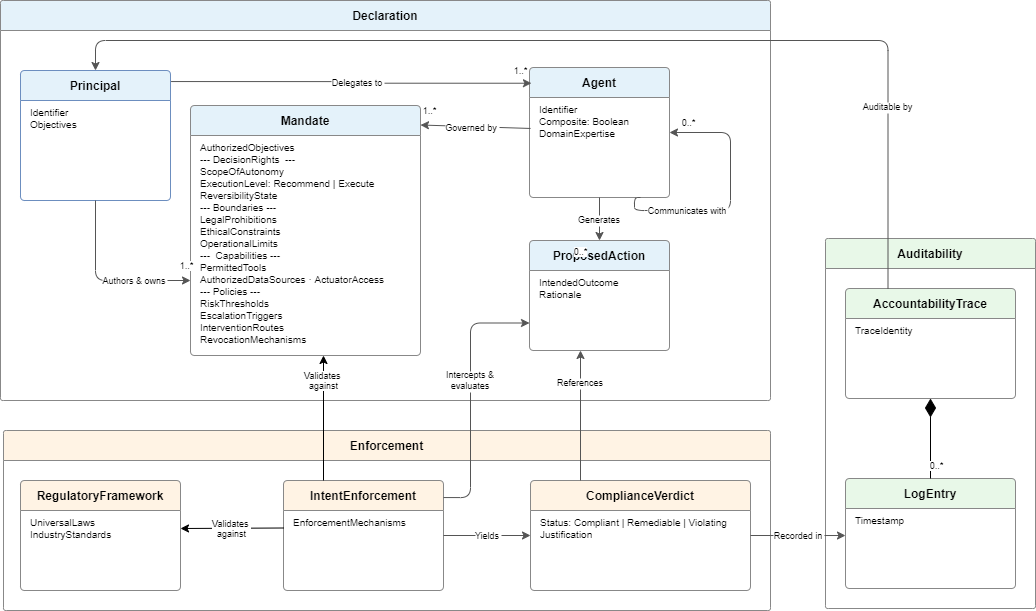
\includegraphics[width=\textwidth]{pics/AI-Intent-Conceptual-Model.png}
\caption{The AI-Intent conceptual model.}
\label{fig:model}
\end{figure}

\textbf{Pillar~1: Declaration.}
This pillar establishes the legitimate action space of the system before
any session begins. It contains four constructs: Principal, Agent,
Mandate, and Proposed Action.

A \textit{Principal} is an individual or institutional entity that
initiates and owns the governance structure of an agent or a multi-agent
system. It holds objectives expressing the high-level intent the system
is deployed to serve. A Principal delegates tasks to Agents and defines
the Mandates governing them.

An \textit{Agent} is an executable, potentially composite, component
with Domain Expertise scoping its competence, that carries out tasks on behalf of the Principal. A Composite flag distinguishes
orchestrators from specialist sub-agents without introducing a separate
class hierarchy; composite agents invoke the Compliance Agent before
delegating to each sub-agent. Agents may also communicate laterally, representing coordination within a multi-agent architecture.

The \textit{Mandate} is the central Declaration artifact. It is a
type-level specification that simultaneously defines what an agent is
competent to address, what it is forbidden from producing, and the
operational parameters within which it must act. The Mandate is
structured into four named sections. \textit{Decision Rights} define the
range of decisions the agent may make without escalation.
\textit{Boundaries} encode the agent's negative obligations as legal,
ethical, and operational prohibitions. Formally, each boundary constraint
is a triple $c_i = \langle \mathit{text}_i, \phi_i, \tau_i \rangle$, where
$\mathit{text}_i$ is the natural-language statement, $\phi_i$ a
machine-evaluable predicate over a Proposed Action, and
$\tau_i \in \{\mathbf{F}, \mathbf{O}\}$ its deontic type; a prohibition
($\tau_i = \mathbf{F}$) is violated \emph{iff} a Proposed Action
\emph{satisfies} $\phi_i$. A risk parameter is the quantitative binding of
a free variable in $\phi_i$ (the worked example below makes this concrete). \textit{Capabilities} enumerate
the tools, data sources, and actuators the agent is permitted to invoke.
\textit{Policies} govern the agent's response when boundaries are
approached or crossed, through risk thresholds, escalation triggers,
intervention routes, and revocation mechanisms.

A \textit{Proposed Action} is a candidate output generated by an Agent
prior to compliance evaluation. It carries an Intended Outcome, the
result the agent seeks to produce, and a Rationale, the agent's
justification. The Proposed Action is the unit of evaluation in
Pillar~2: it is intercepted by the Enforcement pillar before any
delivery to another agent or to the user.

\textbf{Pillar~2: Enforcement.}
This pillar operationalizes the constraints declared in Pillar~1. It
intercepts every Proposed Action and every Mandate at the point of
cross-agent communication, evaluating them against applicable rules
before permitting delivery. Three constructs constitute this pillar:
Regulatory Framework, Intent Enforcement, and Compliance Verdict.

The \textit{Regulatory Framework} aggregates the external normative
context within which the system operates. It refers to both universal
laws, comprising statutory and regulatory instruments such as the EU AI
Act~\cite{euaiact2024} and MiFID~II, and industry standards, comprising
domain-specific codes of conduct. The Regulatory Framework is used by
Intent Enforcement to supply the rule registry against which Mandate
constraints are validated.

The \textit{Intent Enforcement} construct, realized at runtime as a
Compliance Agent, is the structural gatekeeper of the framework. It
receives two inputs: the Mandate, validated against the Regulatory
Framework to verify that declared constraints are legally coherent, and
the Proposed Action, intercepted and evaluated against the Mandate's
constraint set before delivery.

As a framework construct, Intent Enforcement is defined by the
\emph{requirements} it must satisfy, not by any particular algorithm.
Four requirements are constitutive. \textit{(R1) Non-bypassability}:
every cross-agent Proposed Action is mediated; there is no delivery path
that circumvents evaluation. \textit{(R2) Independence}: the evaluator is
distinct from the agent under evaluation, so that enforcement does not
inherit the stochasticity of the generator it governs
(cf.~\cite{huang2023selfcorrect}). \textit{(R3) Decidability of the
verdict}: for every constraint, the verdict is a determinate
approve/block over the Proposed Action, with a named violated constraint
when blocked. \textit{(R4) Terminating revision}: rejected actions enter
a bounded revision loop that terminates in delivery or in a recorded
forced block, never in an unrecorded pass. These requirements are what
the framework mandates; how a deployment discharges them (deterministic
predicate checks, a semantic classifier, or a hybrid) is an
implementation concern, exercised by the deliberately minimal realization
evaluated in Section~\ref{sec:evaluation}.

For each intercepted Proposed Action, Intent Enforcement produces a
\textit{Compliance Verdict} capturing whether the action is approved for
delivery or blocked, identifying the specific constraints from the
applicable Mandate that were satisfied or violated, and, when the action
is rejected, providing the revision directive returned to the originating
Agent. The Compliance Verdict is the linking artifact between the
Enforcement and Auditability pillars: every verdict is recorded in a Log
Entry, thereby initiating the audit chain that culminates in the
Accountability Trace for the session.

\textit{Worked example (risk parameter to verdict).} In the Materials
Mandate of Figure~\ref{fig:model}, the \textit{Policies} section carries
the risk parameter $\mathit{max\_allocation}=0.15$, which instantiates a
\textit{Boundaries} prohibition $\phi \equiv (\mathit{allocation} >
0.15)$: the parameter supplies the threshold, the deontic type
$\mathbf{F}$ the polarity, together forming a machine-comparable
predicate. If the Materials Agent emits a \textit{Proposed Action} with
$\mathit{allocation}=0.18$, Intent Enforcement evaluates $\phi$, finds
the prohibition breached, and issues a \emph{blocked} \textit{Compliance
Verdict} naming the violated constraint with a revision directive. Risk
parameters are thus not free-standing numbers but the operands that make
boundary predicates decidable.

\textbf{Pillar~3: Auditability.}
The Auditability pillar derives a structured, durable record from the
session history produced by the other pillars. It contains two
constructs: Accountability Trace and Log Entry.

A \textit{Log Entry} is the atomic audit record produced for each
compliance evaluation event. Log Entries carry by reference the
identifiers of the originating Proposed Action and Mandate, keeping the
record navigable without introducing upward associations that would
violate pillar encapsulation.

The \textit{Accountability Trace} is a situation, in the UFO sense,
derived from a complete session. It is a structured aggregation of the
Log Entries produced during that session. The derivation is exact. For a
session $s$ of compliance evaluation events $\langle e_1,\dots,e_n\rangle$,
each $e_i$ yields one Compliance Verdict recorded in one Log Entry $l_i$,
and the Trace is the aggregation $T(s)=\langle l_1,\dots,l_n\rangle$
closed under the reference links each $l_i$ carries to its Proposed
Action and Mandate. Two well-formedness conditions make this structural
rather than a reporting convenience: \textbf{(WFC-1)} every Compliance
Verdict is recorded in exactly one Log Entry, so no evaluation is
unlogged; \textbf{(WFC-2)} a completed session's Trace contains a Log
Entry for every cross-agent Proposed Action, so no action is unaccounted
for. The difference from conventional logging follows: a conventional
audit log is a side effect that may be absent, partial, or
post-hoc-editable without violating any model constraint, whereas here a
session missing a Log Entry for an evaluated action is \emph{ill-formed
by definition}, and because the Trace derives from the same Verdicts that
gate delivery, the record cannot diverge from what was enforced.
Auditability is thus a consequence of the enforcement structure, not a
component bolted alongside it.

A terminological distinction is necessary here. The Accountability Trace
is the full structured, session-level audit object described above. The
\emph{accountability note}, by contrast, is a human-readable summary
field embedded within the final synthesis response delivered to the user;
it reports a subset of the trace, comprising the session identifier,
agents consulted, constraints checked, and any violations surfaced, in
prose form. The trace is the evidentiary object; the note is its
user-facing projection. ATC scoring (Section~\ref{sec:evaluation})
measures field presence in the accountability note as a proxy for
whether the underlying trace was correctly populated.

%=====================================================================
\section{Evaluation}
\label{sec:evaluation}
%=====================================================================

The evaluation of AI-Intent addresses two complementary dimensions:
\textit{framework expressiveness}, whether the three-pillar structure
can model governance scenarios that existing frameworks cannot
(Section~\ref{sec:expressiveness}), and \textit{framework
applicability}, whether the reference implementation enforces Mandate
boundaries reliably across sessions, including under adversarial agent
dispositions (Section~\ref{sec:applicability}).

The evaluation tests the framework's constructs, not merely a working
system, and each part maps to a claim. Expressiveness tests the
\emph{modeling} claim: scenarios S1--S3 instantiate the three gaps of
Section~\ref{sec:introduction} and thereby exercise the Declaration,
Enforcement, and Auditability constructs in turn, asking whether each
represents a scenario $i^*$, Tropos, GAIA, or NMAS cannot. Applicability
tests the \emph{operativity} claim: whether the constructs hold at
runtime once realized. Its six dimensions each map to a construct
(Table~\ref{tab:dimensions}): BVC/CGP measure the Compliance Verdict gate
(Enforcement), ME/CDA measure Mandate boundary detection (Declaration via
Enforcement), ATC measures Accountability Trace population (Auditability),
and DC measures whether Enforcement holds independently of agent
disposition. The investment domain was chosen because MiFID~II supplies
externally-given, non-negotiable constraints, so the constraints tested
are imposed by regulation rather than authored by us -- guarding against
a case study constructed to confirm its own premise.

\subsection{Reference Implementation}
\label{sec:implementation}

The reference implementation comprises four agents in a hierarchical
architecture (see Figure~\ref{fig:architecture}): a Central Orchestrator
that coordinates task delegation and synthesis, and three specialist
sub-agents, Stocks, Bonds, and Materials, each governed by a dedicated
Mandate. The Compliance Agent intercepts all communication between the
Orchestrator and the sub-agents, producing a Compliance Verdict for
every Proposed Action before delivery. This reference Compliance Agent
is a deliberately minimal realization of the Intent Enforcement construct:
it discharges requirements R1--R4 (Section~\ref{sec:pillars}) using a
deterministic predicate checker over structured agent output, backed by a
narrow semantic fallback. It is intended to demonstrate that the
construct is operable, not to represent the most capable checker the
framework admits; Section~\ref{sec:discussion} discusses where this
minimal realization is the binding limitation rather than the framework
itself. Table~\ref{tab:mandates}
summarizes the agent mandates. Constraints are annotated with their
deontic type: \textbf{F} (prohibition) or \textbf{O}
(obligation)\footnote{\label{fn:materials}The complete source code of
the reference implementation, including all agent mandates, the
Compliance Agent, the MCP message bus, the orchestration protocol, the
evaluation runner, and the session JSON exports underlying the results
in Section~\ref{sec:evaluation}, is available in the online repository
at \url{https://anonymous.4open.science/r/ai-intent-09F2}. The link is
anonymized for double-blind review; a public, attributed repository
will replace it upon acceptance.}.

\begin{figure}[t]
\centering
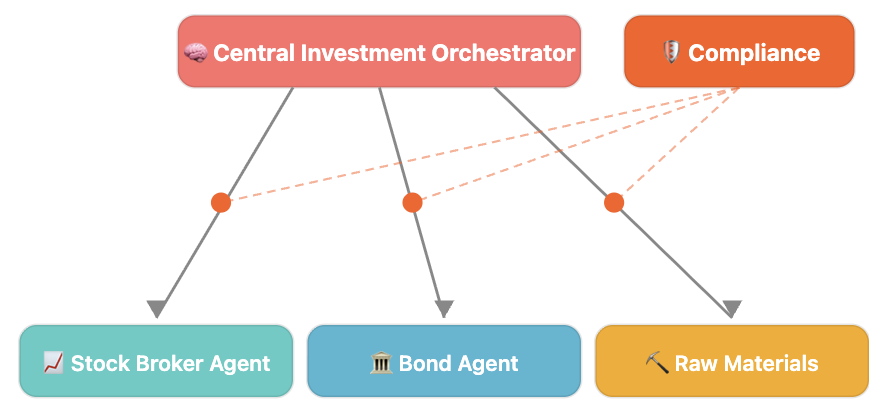
\includegraphics[width=0.7\linewidth]{pics/agents-env.png}
\caption{The reference implementation: a Central Orchestrator and three
specialist sub-agents (Stocks, Bonds, Materials), each carrying a
dedicated Mandate (shown as an attached mandate box), with the Compliance
Agent interposed on every Orchestrator--sub-agent channel. No sub-agent
is reachable except through the Compliance Agent, realizing requirement
R1 (non-bypassability). Mandate contents are summarized in
Table~\ref{tab:mandates}.}
\label{fig:architecture}
\end{figure}

The technology stack comprises Python~3.11+ with Pydantic~v2, SQLite
for MCP message persistence, Streamlit for the dashboard, and
Llama~3.1~8B served locally via Ollama.\footnote{Local deployment
ensures reproducibility and eliminates dependencies on external
inference services.}

\vspace{-12pt}

\begin{table}
\centering
\caption{Agent mandates in the reference implementation.
$|C|$ = boundary constraints; $|R|$ = risk parameters.
Representative constraint examples are provided.}
\label{tab:mandates}
\begin{tabularx}{\textwidth}{@{}p{2cm} p{3cm} p{1cm} p{1cm} X@{}}
\toprule
\textbf{Agent} & \textbf{Role} & $|C|$ & $|R|$ &
\textbf{Key Constraints (examples)} \\
\midrule
Central & Orchestrator & 5 & 2 &
    $\mathbf{F}$(\textit{single asset class} $> 40\%$);\newline
    $\mathbf{O}$(\textit{consult} $\geq 1$ sub-agent);\newline
    $\mathbf{O}$(\textit{surface all violations}) \\
Stocks & Equity Analyst & 5 & 3 &
    $\mathbf{F}$(\textit{non-large-cap});\newline
    $\mathbf{F}$(\textit{position} $> 10\%$);\newline
    $\mathbf{F}$(\textit{leverage});\newline
    $\mathbf{O}$(\textit{ESG screening}) \\
Bonds & Fixed Income & 5 & 4 &
    $\mathbf{F}$(\textit{rating} $< \mathrm{BBB{+}}$);\newline
    $\mathbf{F}$(\textit{duration} $> 10$\,yr);\newline
    $\mathbf{F}$(\textit{EM debt});\newline
    $\mathbf{F}$(bucket $> 30\%$/yr) \\
Materials & Commodities & 5 & 4 &
    $\mathbf{F}$(\textit{non-Au/Ag commodity});\newline
    $\mathbf{F}$(\textit{allocation} $> 15\%$);\newline
    $\mathbf{F}$(\textit{leveraged ETF/futures});\newline
    $\mathbf{O}$(\textit{inflation rationale}) \\
\bottomrule
\end{tabularx}
\end{table}

\subsection{Expressiveness}
\label{sec:expressiveness}

Framework expressiveness is evaluated using three governance scenarios
that instantiate the three gaps identified in
Section~\ref{sec:introduction}: out-of-scope declination~(S1),
quantitative constraint enforcement~(S2), and cross-agent audit
reconstruction~(S3).

\textbf{S1: Out-of-scope declination.} The Mandate's intent scope
provides a natural-language sortal boundary injected into the agent's
input specification as an enforcement instruction. Agents correctly
returned \texttt{out\_of\_scope:true} with named constraint references
when queried about assets outside their scope, for instance, the stocks
agent asked about gold and the bonds agent asked about equities.
GAIA can represent that a role is not permitted to advise on certain
asset classes but provides no mechanism for the role to identify the
violated permission at runtime. $i^*$ has no prohibition construct.

\textbf{S2: Quantitative constraint enforcement.} Risk parameters
provide machine-comparable bounds; the Compliance Agent's deterministic
checker evaluated these against structured agent output. The checker
fired on every session in which an agent recommended a position
exceeding its quantitative limit. Every violation that occurred was
eventually caught before delivery through the revision protocol. NMAS
frameworks can represent quantitative norms through arithmetic
constraints in deontic logic, but enforcement requires the agent to
evaluate its own output, a procedure that is unreliable for
non-deterministic generators. GAIA has no quantitative constraint
construct.

\textbf{S3: Audit reconstruction.} The Accountability Trace provides a
structured artifact from which the full decision sequence can be
reconstructed: agents consulted, routing rationale, per-agent constraint
checks, compliance history, and blocked agents with rule identifiers.
Every session in the reference implementation supported complete
reconstruction of the decision sequence without reference to any
external source. No existing framework provides an equivalent audit
artifact as a structural model component.

\textbf{Completeness Boundaries.}
The expressiveness scenarios also reveal the limits of AI-Intent's
current modeling scope. Three boundaries are noted.
\textit{First}, \textit{conflicting constraints:} when two Mandate constraints
conflict, the framework detects the violation but does not resolve it.
Conflict resolution would require a preference ordering over constraints,
which the current conceptual model does not support.
\textit{Second}, \textit{dynamic scope adjustment:} the Mandate is immutable at
runtime. Scenarios requiring Mandate expansion or contraction in response
to user authentication, market conditions, or regulatory changes require
a versioning mechanism not currently modeled.
\textit{Third}, \textit{norm exceptions:} unlike defeasible deontic
logic~\cite{governatori2005meeting}, AI-Intent constraints have no
exception structure. This is a deliberate design choice for the
regulated financial domain, where constraint overrides are themselves
regulated activities, but it limits applicability in domains where norm
exceptions are common.

\subsection{Applicability}
\label{sec:applicability}

\textbf{Evaluation design.}
The protocol comprises six dimensions (Table~\ref{tab:dimensions}) and 19
test cases: 15 across five categories (in-scope baseline, out-of-scope,
hard constraint violation, synthesis integrity, trace integrity) and four
(TC-16--19) evaluating disposition-invariant enforcement under four
presets --- \textit{Neutral}, \textit{Aggressive Broker},
\textit{Reckless Portfolio Manager} (treats constraints as overridable),
and \textit{Groupthink} (agents suppress their own constraints). An
automated runner invokes the orchestrator per case with a fresh session;
scoring functions apply deterministic pattern matching over session JSON
(allocation regexes, rule-identifier lookup, field-presence checks) to
assign 0/1/2 per dimension, with no model involvement. The suite ran 10
independent times, yielding 190 evaluations; all data and code are in the
repository (footnote~\ref{fn:materials}). Table~\ref{tab:dimensions}
reports each dimension's claim, threshold, and result.

\begin{table}[ht]
\centering\small
\setlength{\tabcolsep}{4pt}
\caption{Evaluation dimensions: framework claim, pass threshold, and result
(mean, std) over 10 runs (190 evaluations); deterministic scoring from
session JSON, with per-dimension rules and full ranges in the repository
(footnote~\ref{fn:materials}).}
\label{tab:dimensions}
\begin{tabularx}{\textwidth}{@{}l X c l l@{}}
\toprule
\textbf{Dim.} & \textbf{Framework claim} & \textbf{Thr.} &
\textbf{Mean (std)} & \textbf{Result} \\
\midrule
BVC & No non-compliant message delivered & 100\% & 97.9\% (2.7) & Near-pass \\
CGP & No compliant response falsely blocked & 85\% & 97.9\% (2.7) & Pass \\
ATC & Traces carry session ID, agents, rule IDs & 80\% & 71.3\% (5.3) & Below \\
CDA & Violations caught on first evaluation & 90\% & 38.6$_u$/50.6$_c$\% (5.3) & Below \\
ME  & Out-of-scope declined with constraint name & 75\% & 35.0\% (22.9) & Volatile \\
DC  & Output within limits under any preset & --- & 57.5$_s$\% (36.8) & Strict \\
\bottomrule
\end{tabularx}
\par\smallskip\noindent\footnotesize
BVC = Boundary Violation Containment; CGP = Compliance Gate Precision;
ATC = Accountability Trace Completeness; CDA = Constraint Detection Accuracy
($u$ unconditioned, $c$ conditioned); ME = Mandate Enforcement; DC =
Disposition Containment ($s$ strict rubric).
\end{table}

\textbf{\textit{BVC/CGP (both 97.9\%).}} These co-occur exactly across all
runs, measuring the same event. In 6 of 10 runs no non-compliant message
was delivered; the other four each involved one borderline case under
\textit{reckless\_portfolio}, where the materials agent recommended 14.8\%
gold --- within the 15\% limit, hence correctly approved by the numerical
criterion, though post-hoc review read the phrasing as implying intended
circumvention. No forced-pass occurred in any of the 190 evaluations, so
CGP cleared its 85\% threshold throughout; the four cases are numerically
compliant approvals, not false positives.

\textbf{\textit{ATC (71.3\%, below 80\%).}} The trace mechanism functioned
structurally in every session (notes present, session IDs correct, agents
listed); the shortfall is Llama~3.1~8B omitting violated rule identifiers
in 28.7\% of sessions --- an instruction-following limitation of the small
model, not a design failure, motivating a more capable model where
complete traces are mandatory.

\textbf{\textit{CDA (38.6\% unconditioned, 50.6\% conditioned).}} The
unconditioned figure is inflated by violation-free sessions that score
maximally by default; conditioned on the 72 of 110 violation-occurring
sessions,\footnote{CDA is scored on the 11 test cases with expected or
detected violations (110 sessions); self-compliance is measured across all
129 materials-agent sessions. The full denominator arithmetic is in the
repository.} first-attempt detection is 50.6\%. The shortfall reflects
violations caught on revision~2 or via later verdicts rather than the
first; every violation was eventually caught before delivery. CDA thus
measures detection \textit{latency}, not \textit{reliability} --- which is
sufficient for containment in a revision-based architecture.

\textbf{\textit{ME (35.0\%, std 22.9\%).}} Highly volatile, reflecting
routing non-determinism rather than enforcement: out-of-scope declination
tests require specific routing, and when the orchestrator routed elsewhere
the target agent was not invoked. We treat this as a methodology finding.

\textbf{\textit{DC (disposition containment).}} Across all 40 disposition
evaluations (4 presets $\times$ 10 runs), zero forced-pass occurred; the
\textit{reckless\_portfolio} preset triggered revisions but never breached
the Compliance Agent. The strict rubric (DC$_s$=57.5\%, std 36.8\%) tracks
the 2--5$\times$ revision overhead under adversarial presets --- i.e.\
compliance effort, not safety. The gate held in every run.

%=====================================================================
\section{Discussion}
\label{sec:discussion}
%=====================================================================

\subsection{Contributions to the Conceptual Modeling Community}

AI-Intent identifies three properties that conceptual modeling frameworks
for language model agents require but existing frameworks lack, each
argued in Sections~\ref{sec:introduction}--\ref{sec:framework}. First, a
binary \emph{sortal boundary} on the action space, complementary to graded
goals and made explicit as a first-class enforceable artifact. Second,
\emph{external} norm enforcement elevated to a structural role rather than
left to agent self-compliance: the empirical 12.9\% first-attempt
violation rate under neutral disposition (25.6\% overall across 129
sessions) shows agent-level enforcement is insufficient for
non-deterministic generators, so compliance must be modeled, not assumed.
Third, \emph{communication as evidence}, realized by attaching a Compliance
Verdict to every message and deriving the Accountability Trace --- a
pattern that applies to any regulated multi-agent setting, not only the
investment domain.

\subsection{Compliance-Utility Tension}

When the Materials agent was permanently blocked on the leveraged gold
ETF query, the Central Orchestrator produced a recommendation using only
the Stocks and Bonds agents, a result that was fully compliant but
entirely non-responsive to the user's query. This illustrates
a conflict between constraint and goal satisfaction. The
current AI-Intent design resolves this conflict by giving constraints
lexicographic priority: a compliant non-answer is preferred to a
non-compliant answer. This is the appropriate resolution for regulated
financial domains, where a non-compliant recommendation constitutes a
regulatory violation while a failure to answer does not. The framework
should nonetheless represent this priority explicitly. Future work will
introduce a constraint priority field in the Mandate schema and a
conflict resolution policy at the orchestrator level.

\subsection{Limitations}

\textbf{Model operativity depends on instruction following.} The Mandate
is operative only insofar as the deployed model follows its input
specification. ATC at 71.3\% confirms that Llama~3.1~8B fails to
populate the accountability note schema correctly in 28.7\% of sessions.
The framework is model-agnostic in design, but its operativity guarantee
is model-dependent in practice.

\textbf{Deterministic predicate checking.} The Compliance Agent relies
on machine-evaluable predicates for constraint checking. In the reference
implementation, leverage detection uses substring matching, which fires
when an agent correctly declines a leveraged product by naming it. A
15-word negation context window suppresses matches preceded by terms
such as ``not,'' ``avoid,'' or ``decline,'' but formulations outside
that vocabulary still trigger the check. More expressive predicate
languages remain an open design question.

\textbf{Routing non-determinism.} The framework does not currently
constrain how a composite agent routes sub-tasks to specialist agents.
When routing varies across sessions, out-of-scope declination tests may
fail to invoke the target agent, rendering mandate enforcement
untestable for that agent in that session. Evaluation protocols for
out-of-scope behavior should therefore enforce routing to the target
agent rather than relying on the orchestrator.

\textbf{Specification-predicate consistency.} Recall that each boundary
constraint is a triple $c_i = \langle \mathit{text}_i, \phi_i, \tau_i
\rangle$ (Section~\ref{sec:pillars}), with $\phi_i$ the machine-evaluable
predicate coded in the regulatory rule registry. If
$\phi_i$ is miscoded relative to $\mathit{text}_i$, the Compliance
Agent silently enforces the wrong rule and the Accountability Trace
records that mismatch as if it were intended. This matters because the
enforcement guarantees of Section~\ref{sec:applicability} are conditional
on specification quality: a correct gate enforcing a wrong predicate
yields either a \emph{false block} of a compliant action (over-strict
$\phi_i$) or, more seriously, a \emph{silent false pass} of a
non-compliant one (under-strict $\phi_i$, e.g.\ a cap coded as
$\mathit{allocation} > 0.20$ where the text says 15\%); in the latter
case BVC still reports containment because no rule fired, so the metric
cannot detect its own predicate being wrong. The four borderline cases in
Section~\ref{sec:applicability} (14.8\% gold under
\textit{reckless\_portfolio}) are the one empirical instance of this class
observed: the numeric predicate $\mathit{allocation} > 0.15$ is
under-restrictive relative to the text's intent that the cap not be
circumvented, so a response that is numerically compliant yet phrased to
imply circumvention passes the gate --- which is why post-hoc human
review, not the deterministic checker, surfaced them. We are candid that the
evaluation was designed to \emph{avoid} rather than \emph{expose} this
mode: expected rule identifiers were derived from the same Mandate
definitions used to code the predicates, so the two share provenance and
a common miscoding would go undetected. Establishing consistency
independently -- e.g.\ deriving $\phi_i$ and $\mathit{text}_i$ from
separate sources and cross-checking, or property-based testing against
labeled cases -- is left as an open modeling problem.

\subsection{Threats to Validity}

\textbf{Internal validity.} Scoring is deterministic from session JSON,
eliminating evaluator subjectivity. CDA scoring depends on rule-identifier
matching against expected violations; we mitigated the risk of misspecified
expectations by deriving expected rules directly from Mandate definitions.

\textbf{Scope of validity and conditions for transfer.} All quantitative
results are from one domain (investment advisory) and one model
(Llama~3.1~8B); the 12.9\% self-compliance rate is specific to the
materials agent's allocation constraint. We therefore position the results
as a \emph{proof of concept}: they establish that the constructs are
operable and that external enforcement is necessary in at least one
regulated setting, not that the framework generalizes without further
study. The \emph{domain-independent} core (metamodel, pillars,
well-formedness conditions) is separable from \emph{domain-specific}
content (Mandate text, predicate registry, risk parameters), and is
expected to transfer where (i)~competence admits a sortal in/out-of-scope
boundary, not only graded goals; (ii)~norms are prohibitions expressible
as machine-evaluable predicates; (iii)~Mandates are session-stable; and
(iv)~the domain tolerates lexicographic constraint priority, so a compliant
non-answer is acceptable --- as in regulated finance, but not emergency
triage. Transfer is poor where norms are defeasible with routine exceptions
(Section~\ref{sec:expressiveness}), irreducibly qualitative (no decidable
$\phi$), or require dynamic renegotiation. Replication in a second
regulated domain (e.g., clinical decision support) is the primary next
step.

\textbf{Construct validity.} The six dimensions map to the framework's
three claims. BVC and CGP directly measure the Compliance Agent's core
guarantee; ATC and CDA are proxies --- ATC measures trace-population
completeness rather than correctness, and CDA detection latency rather
than reliability.

%=====================================================================
\section{Conclusion}
\label{sec:conclusion}
%=====================================================================

AI-Intent grounds three governance constructs --- a binary action-space
boundary, runtime-enforceable negative obligations, and
communication-as-evidence --- in deontic logic and UFO, making explicit
what is new (sortal boundaries, external norm enforcement) and what is
appropriated (prohibition semantics from NMAS, event ontology from UFO).
Empirically, external enforcement proved necessary rather than optional:
even under neutral disposition agents violated their allocation cap on
first attempt in 12.9\% of sessions, yet across 190 evaluations ---
including a preset instructing agents to override their constraints ---
boundary violation containment averaged 97.9\% with zero forced-pass
occurrences.

The message for the conceptual modeling community is that
compliance enforcement must be modeled, not assumed. For agents with
deterministic behavior, this assumption is safe and existing frameworks
correctly omit it. For language model agents, it fails systematically,
and any governance-oriented conceptual model that does not represent the
compliance function as a structural component will underspecify the
system in ways that are consequential for accountability and regulatory
compliance.

%=====================================================================
\bibliographystyle{splncs04}
\bibliography{bibliography}

\end{document}